\chapter{Definicja problemu}\label{chap:problem_definition}

Graf przetwarzania sygnałów można opisać jako zbiór połączonych węzłów generujących
i przetwarzających sygnał dźwiękowy. Każdy węzeł opisany jest poprzez:

\begin{enumerate}
  \item zbiór wejść,
  \item zbiór wyjść,
  \item procedurę obliczeniową wykonywaną na sygnale.
\end{enumerate}


\begin{figure}[H]
  \centering
  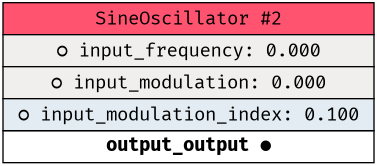
\includegraphics[width=0.4\linewidth]{rys05/example_sine_node.png}
  \caption{Przykładowy węzeł w grafie, generujący sygnał sinusoidalny z możliwością modulacji fazy.}
\end{figure}


\noindent
Przykładowo, dla syntezy subtraktywnej powszechnie wykorzystywane są następujące typy węzłów:

\begin{multicols}{2}

\noindent
\textbf{Oscylator} (\textit{VCO}):
\begin{enumerate}
  \item Wejścia:
    \begin{itemize}
      \item częstotliwość,
      \item kształt fali.
    \end{itemize}
  \item Wyjścia:
    \begin{itemize}
      \item wygenerowany sygnał.
    \end{itemize}
\end{enumerate}

\noindent
\textbf{Filtr} (\textit{VCF}):
\begin{enumerate}
  \item Wejścia:
    \begin{itemize}
      \item sygnał wejściowy
      \item częstotliwość odcięcia,
      \item rezonans.
    \end{itemize}
  \item Wyjścia:
    \begin{itemize}
      \item przefiltrowany sygnał.
    \end{itemize}
\end{enumerate}

\end{multicols}


\section{Budowa grafu}

\begin{figure}[H]\label{fig:example_graph_definition_chapter}
    \centering
    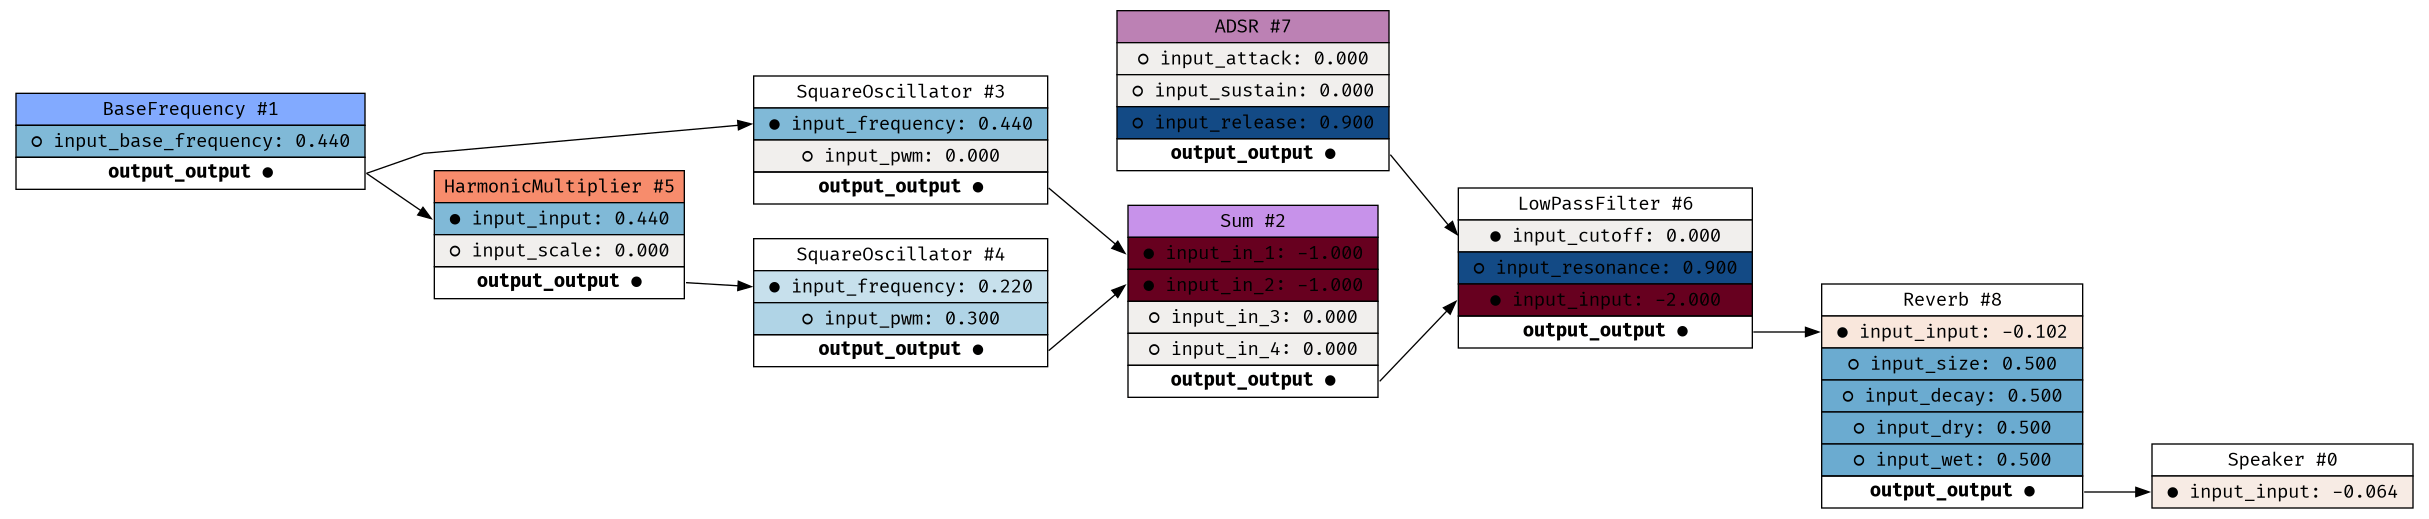
\includegraphics[width=0.9\linewidth]{rys05/luthier_simple_analog.png}
    \caption{
      Przykładowy graf DSP\@. Wolne wejścia, które nie są modulowane przez
      źródła sygnału w grafie są optymalizowanymi parametrami.
    }
\end{figure}


Pełny graf przetwarzania można opisać za pomocą zbioru węzłów oraz
listy połączeń między węzłami:

$N = [n_1, n_2, .., n_n]$ - liczba węzłów,

$i_{j} = [ p_1, p_2, \ldots, p_m ]$ -- Zbiór wejść (\textit{inputs}) j-go węzła. $i_{l, m}$ oznacza $m$-te wejście $l$-go węzła.

$o_{j} = [ p_1, p_2, \ldots, p_m ]$ -- Zbiór wyjść (\textit{outputs}) j-go węzła,

$f_i(x)$ -- operacja wykonywana na sygnale przez i-ty węzeł. % chtex 8

% $C = [ \{ o_{(j, k)}, i_{(l, m)} \}, \ldots ] $: lista połączeń między węzłami, opisujący, które 
$C = [ \{ (j, k), (l, m) \}, \ldots ] $: lista połączeń między węzłami, opisujący, które 
$k$-te wyjście $j$-go węzła podłączone jest do którego $m$-go wejścia $l$-go węzła. Przykładowo,
dla diagramu~\ref{fig:example_graph_definition_chapter}, jednym z połączeń będzie $\{(1, 0), (5, 0)\}$,
ponieważ zerowe wyjście węzła \texttt{BaseFrequency~\#1} podłączone jest do zerowego
wejścia węzła \texttt{HarmonicMultiplier~\#5}.

Nie wszystkie wejścia w grafie muszą być podłączone do któregoś z wyjść, 
co jest widdoczne na diagramie~\ref{fig:example_graph_definition_chapter}.
Wejście, które nie zostało nigdzie podłączone przyjmuje jako wartość wejściową parametr 
liczbowy, optymalizowany na podstawie wartości funkcji celu~(\ref{eq:target_function}).
W~przypadku schematu~\ref{fig:minilogue_diagram} takimi~,,wolnymi'' wejściami są przykładowo
sygnał określający częstotliwość odcięcia filtru sygnału lub parametry określające parametry
generatora obwiedni~(\textit{EG}).
W~pracy wykorzystano algorytm genetyczny \textit{differential evolution}~\cite{2020SciPy-NMeth}
do wygenerowania struktury i parametrów grafu.
Genotyp opisujący dany graf przetwarzania sygnałów składa się z dwóch części:
\begin{enumerate}
  \item fragment decydujący o strukturze grafu, $S = [s_1, s_2,~\ldots]$,
  \item fragment decydujący o wartości parametrów w wolnych wejściach, $P = [p_2, p_2,~\ldots]$.
\end{enumerate}

\subsection{Struktura grafu}\label{sec:graph_structure_definition}

Różne rodzaje syntezy dźwięku wykorzystują różnorodne struktury grafu przetwarzania
sygnałów~\cite{minilogue_diagram}~\cite{digitone_manual}.
Aby umożliwić dostosowanie grafu przetwarzania sygnałów do wykonywania różnych
rodzajów syntezy, struktura grafu przetwarzania sygnałów jest dynamicznie
modyfikowana przez algorytm optymalizacji. Algorytm generujący określoną
strukturę grafu na podstawie genotypu opisany jest w rozdziale~\ref{chap:solution_algorithm}.
Genotyp odpowiadający za strukturę grafu ma formę krotki liczb rzeczywistych $S$.
Praca definiuje funkcję generującą strukturę grafu $G_s$ z genotypu:
\begin{equation}
  G_s(S) = N, C
  \label{eq:graph_structure_generation_function}
\end{equation}

\subsection{Przypisanie parametrów do~,,wolnych wejść''}\label{sec:graph_params_definition}

Po stworzeniu grafu o danej strukturze $G_s$, druga część genotypu wykorzystywana
jest jako wartości poszczególnych parametrów $P$ dla wolnych wejść w grafie przetwarzania
sygnału.

\begin{equation}
  \forall_{(l,m)} (l, m) \notin C, i_{l,m} = P_j
  \label{eq:graph_params_assignment}
\end{equation}

\section{Funkcja celu}

Wykorzystana w pracy funkcja celu $F$, oceniająca, jak sygnał wygenerowany ($\bar{x}$) przez algorytm
jest bliski sygnałowi docelowemu ($x$) przedstawiona jest w następujący sposób:

\begin{equation}
  F(x, \bar{x}) = DTW(MFCC(x),~MFCC(\bar{x}))
  \label{eq:target_function}
\end{equation}

\noindent
Gdzie $MFCC$ oznacza \textit{mel-frequency cepstrum coefficients}~(\ref{fig:mfcc_calculation_diagram}),
natomiast $DTW$ oznacza algorytm \textit{dynamic time warping}~\cite{mfcc_dtw}.
Uzasadnienie wybranej funkcji celu opisane jest w rozdziale~\ref{target_function_chapter}.

\subsection{Wyliczanie współczynników MFCC~\cite{kacprzak2010inteligentne}}

\begin{figure}[H]\label{fig:mfcc_calculation_diagram}
\centering

\begin{tikzpicture}[node distance=2cm]
\node (signal) [startstop] {Sygnał dźwiękowy};
\node (preemphasis) [process, right of=signal, xshift=2cm] {Preemfaza};
\node (windowing) [process, right of=preemphasis, xshift=2cm] {Ramkowanie i okienkowanie};
\node (ffts) [process, right of=windowing, xshift=2cm] {$|FFT|^2$};
\node (mel) [process, below of=signal] {zestaw filtrów w skali \textit{MEL}};
\node (log) [process, right of=mel, xshift=2cm] {skala \\ logarytmiczna};
\node (dct) [process, right of=log, xshift=2cm] {dyskretna transformata cosinusowa};
\node (mfcc) [startstop, right of=dct, xshift=2cm] {Współczynniki MFCC};

\draw [arrow] (signal) -- (preemphasis);
\draw [arrow] (preemphasis) -- (windowing);
\draw [arrow] (windowing) -- (ffts);
\draw[thick, ->,rounded corners] (ffts) |- node[fill=white,inner sep=2pt]{} ++(-12,-1) -- (mel);
\draw [arrow] (mel) -- (log);
\draw [arrow] (log) -- (dct);
\draw [arrow] (dct) -- (mfcc);
\end{tikzpicture}
  \caption{Schemat algorytmu obliczania współczynników MFCC,
  zaczerpnięty z~\cite{kacprzak2010inteligentne}.
  Praca wykorzystuje gotową implementację algorytmu obliczającego współcznyniki MFCC z pakietu \texttt{librosa}~\cite{librosa}.}
\end{figure}

Algorytm obliczania współczynników MFCC przedstawiony jest na rysunku~\ref{fig:mfcc_calculation_diagram}.
Pierwszym krokiem w algorytmie jest zastosowanie preemfazy, która wzmacnia składowe wysokoczęstotliwościowe
i osłabia składowe niskoczęstotliwościowe:

\begin{equation}
  x^\prime_n = x_n - a~x_{n-1}
  \label{eq:preemphasis}
\end{equation}

\noindent
W następnym kroku sygnał jest ramkowany, na każdą ramkę nakładane jest okno Hamminga:

\begin{equation}
  Ham(N) = 0.54 - 0.46 \cos(2\pi \frac{n-1}{N-1})
  \label{eq:hamming_window}
\end{equation}

Dla każdej ramki wyliczana jest transformata Fouriera, aby
obliczyć widmo mocy sygnału $|FFT|^2$. Widmo przetwarzane jest
przez zbiór filtrów $H_m$, których środki są rozmieszczone
w równomiernych odstępach w skali mel. Typ i liczba filtrów zależy
od implementacji algorytmu (w pracy wykorzystano~\cite{librosa}).
Wyjście każdego z filtrów wykorzystane
jest do obliczenia energii przefiltrowanego pasma:

\begin{equation}
  S_m = \sum_{k=1}^{N}| X_r(k) |^2 H_m(k),
  \label{eq:band_energy}
\end{equation}

\noindent
gdzie $X_r$ oznacza widmo danej ramki, $m$ jest numerem filtra.

W ostatnim kroku do obliczenia wartości współczynników MFCC
wykorzystuje się dyskretną transformatę kosinusową.
Aby lepiej przybliżyć wrażliwość ludzkiego ucha na głośność dźwięku,
wykorzystuje się logarytm energii pasma:

\begin{equation}
  c_i = \sqrt{\frac{2}{M}} \sum_{m_1}^{M} \log(S_m) \cos( \frac{\pi i}{M}(M - 0.5) ),
  \label{eq:mfcc_coefficients}
\end{equation}

Gdzie M to liczba użytych filtrów w zbiorze~\ref{eq:band_energy},
a $i$ jest numerem współczynnika.


\section{Ograniczenia}

W algorytmach DSP powszechnie wykorzystuje się ograniczenie wartości
sygnału do przedziału $(-1.0, 1.0)$, gdy implementacja danego algorytmu wykorzystuje 
typ \texttt{float} do przechowywania wartości sygnałów. Środowisko zaimplementowane
w ramach pracy oczekuje, że wartości sygnałów i parametrów sterujących
będą znajdowały się w tym przedziale:

\begin{equation}
  \forall p_j \in P,  -1.0 \leq p_j \leq 1.0, \quad \forall s_i \in S, -1.0 \leq s_i \leq 1.0
  \label{eq:parameter_bounds}
\end{equation}

\section{Problem optymalizacji}

Sygnał wygenerowany przez graf przetwarzania sygnałów zależy od następujących parametrów:

\begin{equation}
  \bar{x} = G(G_s(S), P)
  \label{eq:graph_generated_signal}
\end{equation}

\noindent
Gdzie $G$ jest funkcją generującą sygnał dźwiękowy dla konkretnej struktury grafu
$G_s$~(\ref{sec:graph_structure_definition},~\ref{eq:graph_structure_generation_function}),
dla wartości parametrów przypisanych z
$P$~(\ref{sec:graph_params_definition},~\ref{eq:graph_params_assignment}).
Dla parametrów $S$ oraz $P$, ograniczonych przez~\ref{eq:parameter_bounds},
rozwiązywany jest problem optymalizacyjny:

\begin{equation}
  \text{Minimize}~F(x,~G(G_s(S), P))
  \label{eq:target_function}
\end{equation}

